\documentclass[letterpaper,12pt]{extarticle}
\usepackage{astro-mini}
\usepackage{lipsum}

\usepackage{array}
\newcolumntype{L}{>{$}l<{$}}
\newcolumntype{C}{>{$}c<{$}}
\newcolumntype{R}{>{$}r<{$}}

\begin{document}

\begin{center}

    \Large Laboratorio 9: Variabilidad de Gamma Cassiopeiae: identificación de grupos de frecuencia

    \vspace{3mm}

    \large Juan David Aparicio Gutiérrez

    \vspace{3mm}
    \normalsize
\end{center}


\section{Introducción}

Las estrellas Be son estrellas de tipo espectral B, no supergigantes, que rotan muy rápido —típicamente al 70--100\% de su velocidad crítica— y presentan en algún punto de su vida una o más líneas de Balmer en emisión \cite{sabogal2014}. Dicha emisión proviene de un disco circumestelar de decrecimiento (CDD), formado por gas expulsado desde la superficie estelar \cite{rivinius2013}. A pesar de haber sido descubiertas en 1866 por Angelo Secchi en $\gamma$~Cassiopeiae, los mecanismos que mantienen el disco no están aún completamente comprendidos \cite{sabogal2014}.

La variabilidad fotométrica de las estrellas Be actúa en tres escalas: corto plazo (horas a días, pulsaciones y rotación), medio plazo (semanas a meses, ondas de densidad en el disco) y largo plazo (años a décadas, cambios estructurales del CDD) \cite{sabogal2014}. En el espectro de potencia, la firma más característica es la presencia de \textit{grupos de frecuencia}: señales periódicas cercanas cuya amplitud varía con el tiempo. Con datos de TESS, \cite{labadiebartz2022} encontraron grupos de frecuencia en el 87\% de una muestra de 430 estrellas Be. Los modos g predominan entre $0.5$ y $6\,\mathrm{d}^{-1}$, los modos p entre 6 y $15\,\mathrm{d}^{-1}$, y señales estocásticas de baja frecuencia aparecen en el $\sim$25\% del catálogo \cite{labadiebartz2022}. En estrellas Be de tipo temprano con estructura armónica, los dos grupos principales satisfacen $f_{\rm G2}/f_{\rm G1} \approx 2.0$.

Gamma Cassiopeiae ($\gamma$~Cas, HD~5394), de tipo espectral B0.5~IVe, es la estrella Be más brillante del cielo norte y el prototipo histórico de la clase. Su curva de luz exhibe variabilidad en múltiples escalas, lo que la convierte en un objeto de referencia para probar métodos de análisis espectral de series de tiempo irregulares.


\section{Objetivos}

\begin{itemize}
    \item Construir el periodograma de Lomb-Scargle de $\gamma$~Cas e identificar los grupos de frecuencia significativos, caracterizando cada uno por su frecuencia central $f_c$, anchura $\sigma$ y amplitud mediante ajuste gaussiano.
    \item Evaluar el cociente $f_{\rm G2}/f_{\rm G1}$ y contrastarlo con el valor esperado $\approx 2.0$ para estrellas Be de tipo temprano con estructura armónica de modos g \cite{labadiebartz2022}.
    \item Interpretar físicamente los grupos detectados en términos de pulsaciones no radiales o variabilidad del disco, siguiendo las clasificaciones de \cite{labadiebartz2022} y \cite{sabogal2014}.
    \item Calibrar el umbral FAP y la separación mínima entre picos para maximizar la detección de grupos reales sin generar falsas detecciones por encadenamiento de ruido.
\end{itemize}


\section{Procedimiento}

\subsection{Periodograma de Lomb-Scargle}

Dado que los datos fotométricos provienen de observaciones terrestres con ventanas diurnas y estacionales, la distribución temporal de las mediciones es irregularmente espaciada. El uso de la Transformada de Fourier Discreta estándar introduciría \textit{aliasing} severo bajo estas condiciones. Se emplea en cambio el periodograma de Lomb-Scargle \cite{lomb_1976,scargle_1982}, que ajusta por mínimos cuadrados un modelo sinusoidal flotante en cada frecuencia de prueba $f$, cuya potencia normalizada queda definida en la expresión~\ref{eq:ls}.

\begin{equation}
    P_{\rm LS}(f) = \frac{1}{2}\left[
        \frac{\left(\displaystyle\sum_j h_j \cos 2\pi f(t_j-\tau)\right)^2}
             {\displaystyle\sum_j \cos^2 2\pi f(t_j-\tau)}
      + \frac{\left(\displaystyle\sum_j h_j \sin 2\pi f(t_j-\tau)\right)^2}
             {\displaystyle\sum_j \sin^2 2\pi f(t_j-\tau)}
    \right]
    \label{eq:ls}
\end{equation}

En la expresión~\ref{eq:ls}, $h_j$ es la magnitud medida en el instante $t_j$, y $\tau$ es el desfase que hace el estimador invariante a traslaciones temporales. Dicho desfase se obtiene implícitamente de la relación~\ref{eq:tau}.

\begin{equation}
    \tan(4\pi f\tau) = \frac{\displaystyle\sum_j \sin(4\pi f t_j)}{\displaystyle\sum_j \cos(4\pi f t_j)}
    \label{eq:tau}
\end{equation}

La grilla de frecuencias se construyó con \texttt{LombScargle.autopower} de \texttt{astropy}, con $f_{\min} = 1/T$ (resolución de Rayleigh), $f_{\max} = 9\,\mathrm{d}^{-1}$ y 10 muestras por pico, donde $T$ es la línea de base total de la serie.

\subsection{Umbral de significancia por probabilidad de falsa alarma}

El nivel de potencia correspondiente a una probabilidad de falsa alarma $\alpha$ se obtiene a partir de la distribución del periodograma bajo la hipótesis nula de ruido puro. La probabilidad acumulada para un umbral de potencia $z$ puede aproximarse según la ecuación~\ref{eq:fap}.

\begin{equation}
    \mathrm{FAP}(z) \approx 1 - \left(1 - e^{-z}\right)^{N_{\rm eff}}
    \label{eq:fap}
\end{equation}

En la ecuación~\ref{eq:fap}, $N_{\rm eff}$ es el número efectivo de frecuencias independientes del periodograma. Se utilizó la implementación analítica de \texttt{astropy} con $\alpha = 5\times10^{-3}$, valor resultado del proceso de calibración descrito en la Sección~\ref{sec:problemas}.

\subsection{Detección y agrupamiento de picos}

Los máximos locales por encima del umbral FAP se identificaron con \texttt{scipy.signal.find\_peaks}, exigiendo que la separación entre picos consecutivos cumpla la condición mínima establecida en la ecuación~\ref{eq:dfmin}.

\begin{equation}
    \Delta f_{\min} = 0.01\,\mathrm{d}^{-1}
    \label{eq:dfmin}
\end{equation}

La restricción de la ecuación~\ref{eq:dfmin} evita que múltiples muestras de un mismo pico físico sobre una malla densa sean tratadas como señales independientes. Los picos detectados se agrupan entonces por proximidad según el criterio de la ecuación~\ref{eq:gap}: dos picos sucesivos $f_i < f_{i+1}$ pertenecen al mismo grupo si su separación es inferior a $\Delta f_{\rm gap}$.

\begin{equation}
    f_{i+1} - f_i < \Delta f_{\rm gap} = 0.3\,\mathrm{d}^{-1}
    \label{eq:gap}
\end{equation}

Cuando la separación excede $\Delta f_{\rm gap}$ de la ecuación~\ref{eq:gap}, se inicia un nuevo grupo. Este criterio reproduce conceptualmente el algoritmo de \textit{clustering} por cercanía descrito en el Apéndice~A de \cite{labadiebartz2022}, en el que las frecuencias individuales recuperadas mediante \textit{pre-whitening} iterativo se agregan en grupos según su separación relativa.

\subsection{Caracterización gaussiana de cada grupo}

Para caracterizar espectralmente cada grupo, se ajusta el perfil gaussiano de la expresión~\ref{eq:gauss} sobre la ventana espectral del grupo mediante \texttt{scipy.optimize.curve\_fit}.

\begin{equation}
    G(f) = A\,\exp\!\left[-\frac{(f - f_c)^2}{2\sigma^2}\right]
    \label{eq:gauss}
\end{equation}

Los parámetros resultantes de la expresión~\ref{eq:gauss} son la frecuencia central $f_c$, la anchura espectral $\sigma$ y la amplitud $A$. En caso de no convergencia del ajuste, el centro se estima como el centroide ponderado por la potencia.


\section{Problemas presentados y soluciones aplicadas}
\label{sec:problemas}

El principal desafío del análisis fue la calibración simultánea del umbral FAP y la separación mínima entre picos detectados. Con el valor inicial $\alpha = 10^{-4}$, el nivel de significancia resultó demasiado elevado: un grupo visualmente distinguible en el periodograma, con potencia máxima $\approx 0.0068$, quedaba por debajo del umbral y no era detectado por el algoritmo.

Al relajar el umbral a $\alpha = 10^{-2}$ (1\%), el problema opuesto se presentó con mayor severidad. Dado que la separación mínima entre picos era de apenas un bin espectral ($\Delta f_{\min} \approx \delta f_{\rm Rayleigh} \sim 10^{-4}\,\mathrm{d}^{-1}$), se detectaron miles de picos adyacentes en la región de baja frecuencia, todos separados por menos de $0.3\,\mathrm{d}^{-1}$, encadenándose en un único megagrupo de 1746 picos que absorbía la totalidad del espectro.

La solución adoptada fue doble: (1)~se fijó $\alpha = 5\times10^{-3}$, valor intermedio que sitúa el umbral por debajo de los picos del grupo débil sin inundar el espectro; y (2)~se impuso $\Delta f_{\min} = 0.01\,\mathrm{d}^{-1}$ como separación mínima entre picos, lo que limita la densidad de detecciones a un máximo de $\sim 100\,\mathrm{d}$ por unidad de frecuencia y elimina el efecto de encadenamiento. Con esta configuración se recuperaron los dos grupos de frecuencia de manera estable.


\section{Resultados}

Se analizó la serie de tiempo fotométrica de $\gamma$~Cas, cuya curva de luz cruda se muestra en la figura~\ref{fig:timeseries}. La variabilidad es marcadamente irregular con fluctuaciones de gran amplitud sobre múltiples escalas temporales, comportamiento típico de las estrellas Be con disco activo.

\begin{figure}[H]
    \centering
    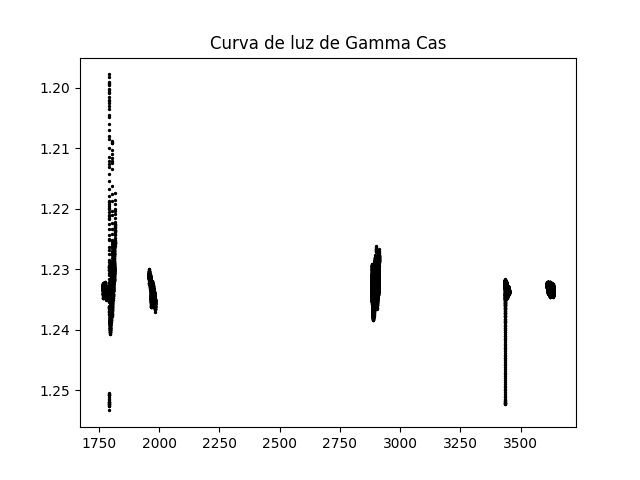
\includegraphics[width=\textwidth]{img/gamma_cas_serie_de_tiempo.png}
    \caption{Serie de tiempo fotométrica de $\gamma$~Cas (datos crudos).}
    \label{fig:timeseries}
\end{figure}

El periodograma de Lomb-Scargle con los grupos de frecuencia detectados se presenta en la figura~\ref{fig:grupos}. Se identificaron 2 grupos significativos; sus parámetros se resumen en la tabla~\ref{tab:grupos}.

\begin{figure}[H]
    \centering
    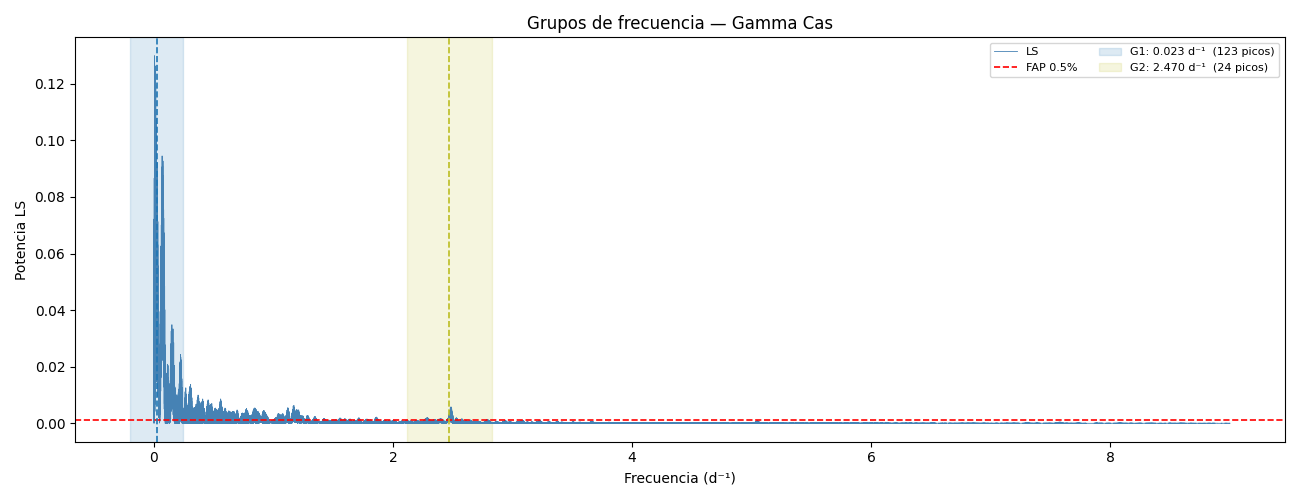
\includegraphics[width=\textwidth]{img/grupos_de_frecuencia_gamma_cas.png}
    \caption{Periodograma de Lomb-Scargle de $\gamma$~Cas. La línea roja discontinua indica el umbral FAP $= 0.5\%$. Las regiones sombreadas corresponden a los intervalos $[f_c - 3\sigma,\, f_c + 3\sigma]$ de cada grupo; las líneas verticales punteadas señalan las frecuencias centrales $f_c$.}
    \label{fig:grupos}
\end{figure}

\begin{table}[H]
    \centering
    \caption{Parámetros de los grupos de frecuencia detectados en $\gamma$~Cas.}
    \label{tab:grupos}
    \begin{tabular}{lcccc}
        \hline\hline
        Grupo & $f_c$ ($\mathrm{d}^{-1}$) & $P_c = 1/f_c$ (d) & $\sigma$ ($\mathrm{d}^{-1}$) & $N_{\rm picos}$ \\
        \hline
        G1 & 0.0234 & 42.7 & 0.0740 & 123 \\
        G2 & 2.4702 & 0.405 & 0.1184 &  24 \\
        \hline
    \end{tabular}
\end{table}

El cociente entre las frecuencias centrales resulta $f_{\rm G2}/f_{\rm G1} = 105.69$, muy alejado del valor $\approx 2.0$ que \cite{labadiebartz2022} reportan para estrellas Be de tipo temprano con estructura armónica de grupos de modos~g. Esta discrepancia es indicativa de que G1 y G2 no forman un par armónico, sino que son originados por mecanismos físicos distintos.


\section{Conclusiones}

El periodograma de $\gamma$~Cas revela dos grupos de frecuencia con características bien distintas entre sí.

El grupo G2 ($f_c = 2.470\,\mathrm{d}^{-1}$, $P \approx 0.41\,\mathrm{d}$) cae dentro del rango típico de los modos g en estrellas Be de tipo temprano ($0.5$--$6\,\mathrm{d}^{-1}$; \cite{labadiebartz2022}), con una anchura $\sigma = 0.118\,\mathrm{d}^{-1}$ consistente con la multipericidad propia de estos grupos. Su interpretación como pulsación no radial de tipo g es consistente con el tipo espectral B0.5~IVe y con la presencia de este tipo de modos en el 87\% de la muestra de TESS reportada por \cite{labadiebartz2022}.

El grupo G1 ($f_c = 0.023\,\mathrm{d}^{-1}$, $P \approx 42.7\,\mathrm{d}$) corresponde a variabilidad de baja frecuencia, en la categoría de tendencias de largo plazo ($f < 0.5\,\mathrm{d}^{-1}$) presentes en el $\sim$25\% del catálogo TESS \cite{labadiebartz2022}. Refleja probablemente cambios en el CDD de $\gamma$~Cas, cuya actividad de formación y disipación opera en escalas de semanas a meses \cite{sabogal2014}.

El cociente $f_{\rm G2}/f_{\rm G1} = 105.69 \gg 2$ confirma que los grupos no son armónicos y que el espectro de $\gamma$~Cas combina variabilidad de disco de largo plazo con pulsaciones g de frecuencia media, en lugar de la estructura de dos grupos de modos g esperada para estrellas Be de tipo temprano \cite{labadiebartz2022}. En cuanto a la metodología, el umbral FAP y la separación mínima entre picos deben calibrarse conjuntamente: valores demasiado estrictos pierden grupos débiles, mientras que valores demasiado laxos provocan encadenamiento de ruido. La configuración $\alpha = 5\times10^{-3}$, $\Delta f_{\min} = 0.01\,\mathrm{d}^{-1}$ resultó adecuada para este conjunto de datos.


% Bibliography
\footnotesize

\bibliographystyle{aa_url}
\bibliography{global.bib}

\end{document}
